\chapter{Konsolenausgaben}

\section{Master Boot Record}

\subsection{Sleutkit}

\begin{itemize}
\item 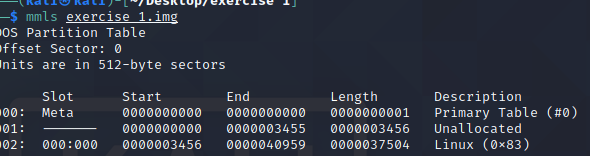
\includegraphics[scale=0.6]{bilder/partition_table.png } 
\item 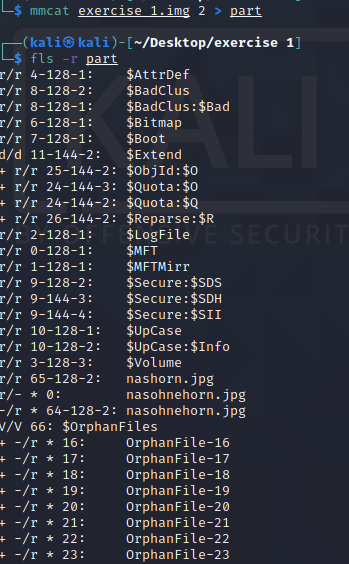
\includegraphics[scale=0.6]{bilder/analyse_Dateisystem.png } 
\item 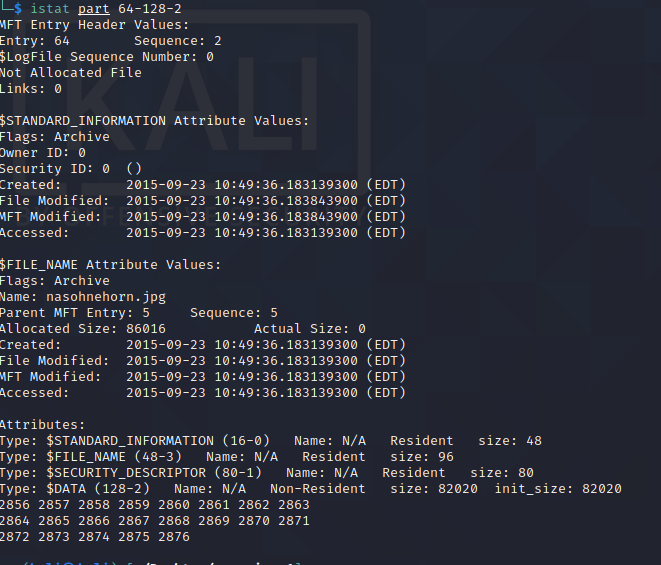
\includegraphics[scale=0.6]{bilder/nasohnehorn_istat.png } 
\item 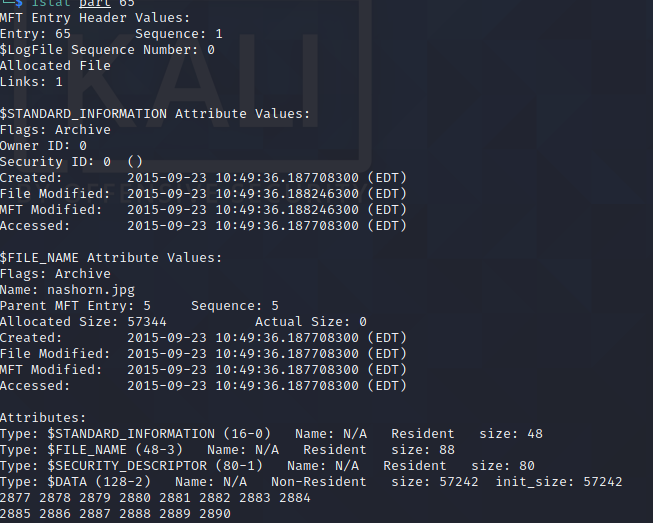
\includegraphics[scale=0.6]{bilder/nashorn_istat.png }
\item TODO HASHES
\end{itemize}

\subsection{Testdisk}

Testdisk wurde mit No Partition und unkown Filesystem verwendet und nach Funde des ersten NTFS wurde mit Deeper Search die drei NTFS gefunden.\\
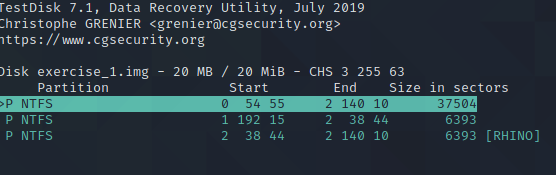
\includegraphics[scale=0.6]{bilder/3_Ntfs_Testdisk.png } \\
Auflisten der Dateien:
\begin{itemize}
\item \includegraphics[scale=0.6]{bilder/first_Ntfs.png } 
\item \includegraphics[scale=0.6]{bilder/second_Ntfs.png } 
\item \includegraphics[scale=0.6]{bilder/third_Ntfs.png } 
\end{itemize}

\subsection{File Carving}
Photorec wurde mit den Standardeinstellungen mit auf No Partition mit Other filesystem types als ext2/ext3/ext4  verwendet.\\
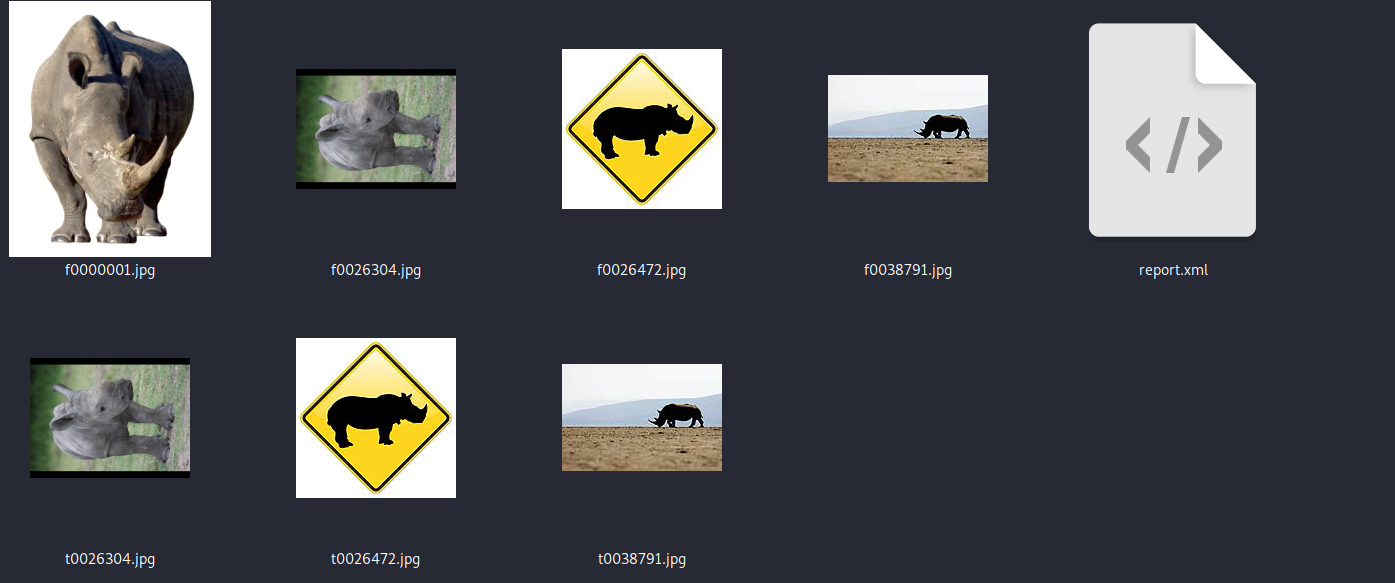
\includegraphics[scale=0.25]{bilder/photorec.png }
